\subsection*{Classifying held-out samples}
In leave-one-out cross-validation, TabPFN, logistic regression and the random forest each classified \mlBinTabpfnFiftyCorrect{} held-out samples correctly as simulated microgravity or static 1g, with either feature count (balanced accuracy \mlBinTabpfnFiftyBal; Fig.~\ref{fig:fig4}a). Every model misclassified the same two samples: \mlBinMisclassified. These are the clinostat sample that lay between the groups in the PCA and the ground sample furthest from the others on PC2. Exact permutation tests show that this accuracy is not clearly better than chance with eight samples (balanced-accuracy $p=\mlBinPMin$--$\mlBinPMax$). However, the held-out probabilities ranked the samples well (AUROC \mlBinAurocMin--\mlBinAurocMax; $p=\mlBinPAuroc$, the smallest attainable), which points to a real but modest separation. On the three-class task, TabPFN classified \mlThreeTabpfnFiftyCorrect{} samples correctly (balanced accuracy \mlThreeTabpfnFiftyBal, $p=\mlThreeTabpfnFiftyP$), where logistic regression (\mlThreeLogregFiftyCorrect) and the random forest (\mlThreeForestFiftyCorrect) were no better than chance (Fig.~\ref{fig:fig4}b). The advantage did not survive adding the inferred RFPRPM4 library (TabPFN \mlSensThreeTabpfnFiftyCorrect, $p=\mlSensThreeTabpfnFiftyP$). Given that, and the many comparisons made, we do not take it as evidence that the two simulators can be told apart.

\begin{figure*}[t]
\centering
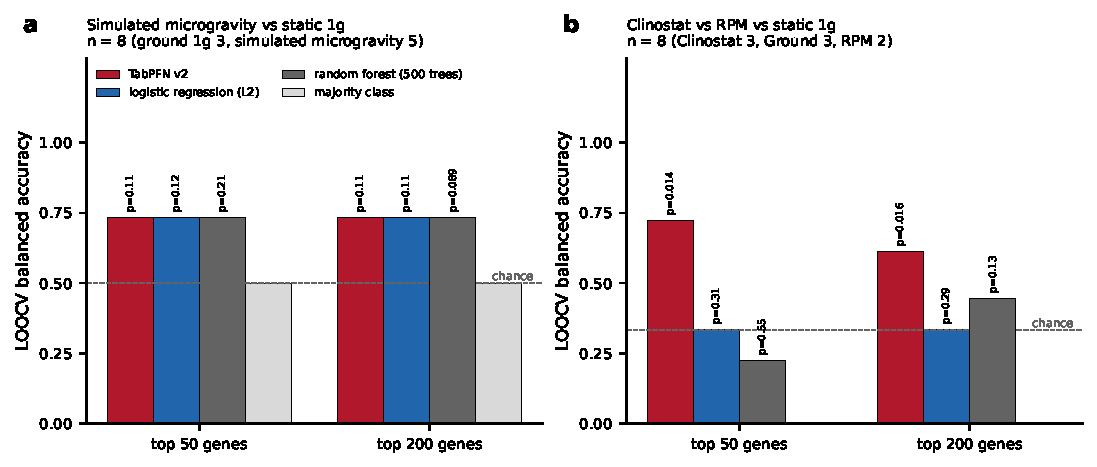
\includegraphics[width=0.95\textwidth]{figures/fig4_classification}
\caption{\textbf{Leave-one-out classification of held-out samples.} Balanced accuracy of TabPFN~v2, L2 logistic regression, a 500-tree random forest and a majority-class baseline, using the top 50 or 200 most variable genes chosen within each training fold. \textbf{a}, Simulated microgravity vs static 1g. \textbf{b}, Clinostat vs RPM vs static 1g. Labels give exact permutation p-values for balanced accuracy (all class-size-preserving relabellings); dashed line, chance (1/number of classes).}
\label{fig:fig4}
\end{figure*}

\subsection*{Metabolic subsystems}
Re-mapping the earlier reaction set to KEGG-supported genes changed it substantially: \keggOldWrong{} of its \keggOldReactions{} reactions had been placed on the wrong gene (Methods). Of the \keggSubsystems{} subsystems, \nSubsystemsSig{} was enriched for DEGs in either contrast: cellular respiration under the RPM. There, \respDegRpm{} tested genes were DEGs, \respUpRpm{} of them up, with a median shrunk $\log_2$ fold change of \respMedianRpm{} (FDR $=\respFdrRpm$; Fig.~\ref{fig:fig9}). Under the clinostat the same subsystem moved in the same direction without reaching significance (\respDegClino{} DEGs, median \respMedianClino, FDR $=\respFdrClino$). The signal comes from the complex~I (\textit{nuo}) genes already seen in the GO analysis. Mycolic acid and FAS-II genes (\mycolicDegClino{} DEGs under the clinostat, \mycolicDegRpm{} under the RPM) and redox and cofactor genes (\redoxDegClino{} and \redoxDegRpm) did not change.

\begin{figure*}[t]
\centering
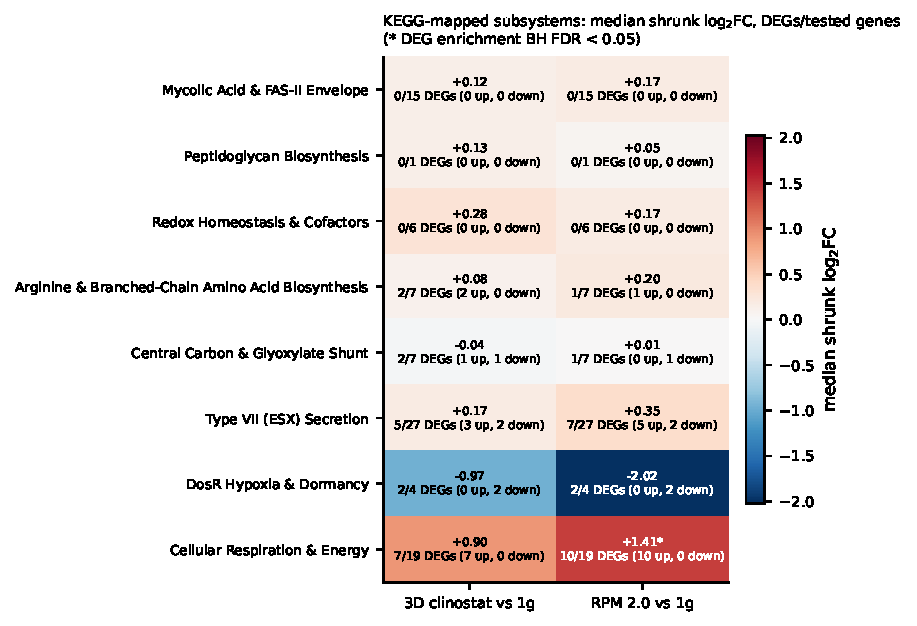
\includegraphics[width=0.7\textwidth]{figures/fig9_metabolic_subsystems}
\caption{\textbf{KEGG-mapped metabolic subsystems.} For each subsystem and contrast: median apeglm-shrunk $\log_2$ fold change across tested genes (colour, first line), and DEGs among tested genes with their direction (second line). *, hypergeometric DEG enrichment with BH FDR $<0.05$.}
\label{fig:fig9}
\end{figure*}

\subsection*{OSD-528 among microbial OSDR studies}
OSDR holds \nOsdrStudies{} microbial spaceflight or simulated-microgravity studies: \nOsdrSpaceflight{} spaceflight studies and \nOsdrGroundSim{} ground simulations (Fig.~\ref{fig:fig7}). They cover bacteria (\nOsdrBacteria{} studies), microbial communities (\nOsdrCommunity) and fungi (\nOsdrFungi). Judged by their recorded factors, \osdrRpmClinostatStudies{} is the only one that pairs an RPM with a 3D clinostat, which makes it the only direct test of these two simulator types in a microbe in the repository.

\begin{figure*}[t]
\centering
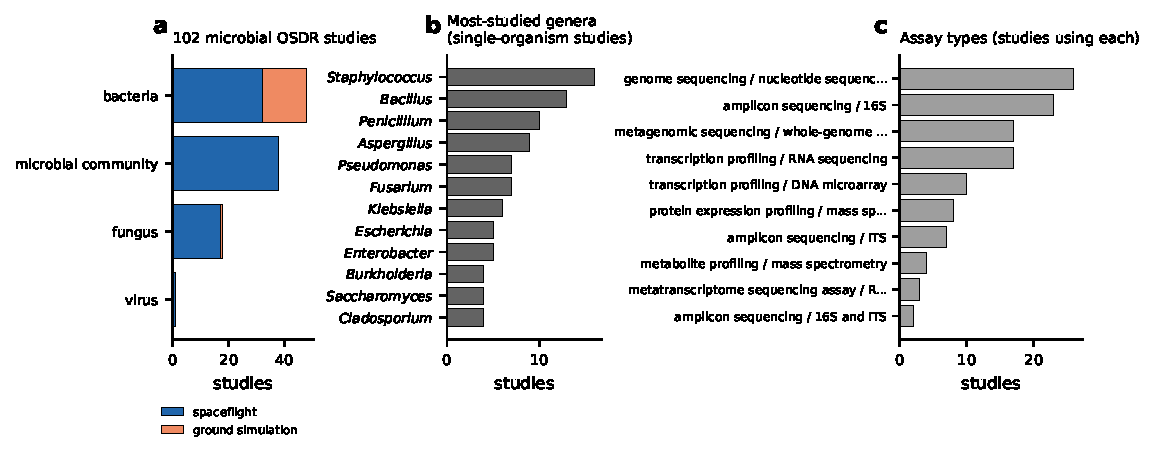
\includegraphics[width=0.95\textwidth]{figures/fig7_osdr_microbial_compendium}
\caption{\textbf{Microbial spaceflight and simulated-microgravity studies in NASA OSDR.} \textbf{a}, Studies per microbial category, split into spaceflight studies and ground simulations (a study can list more than one category). \textbf{b}, The most-studied genera among single-organism studies. \textbf{c}, Assay types, counted once per study. Source: Supplementary Table~S16, built from the OSDR API.}
\label{fig:fig7}
\end{figure*}
